\documentclass[11pt]{article}

% Venue toggles.
% Default behavior is arXiv-portable generic article formatting.
% Uncomment one venue toggle and optionally camera-ready for submission builds.
\newif\ifvenueset
\newif\ifneuripsvenue
\newif\ificmlvenue
\newif\ifcameraready
\venuesetfalse
\neuripsvenuefalse
\icmlvenuefalse
\camerareadyfalse
%
% Examples:
% \neuripsvenuetrue
% \camerareadytrue
%
% \icmlvenuetrue
% \camerareadytrue
%
% External wrapper overrides (used by CI/release builds):
\ifdefined\buildneurips\neuripsvenuetrue\fi
\ifdefined\buildicml\icmlvenuetrue\fi
\ifdefined\buildcameraready\camerareadytrue\fi

% arXiv metadata
\newcommand{\arxivprimaryclass}{cs.AI}
\newcommand{\paperkeywords}{constitutional AI, AI governance, multi-agent systems, fail-closed enforcement, formal verification, long-context systems}
\newcommand{\papertitle}{ACGS: A System-Centric Architecture for Constitutional AI Governance}
\newcommand{\papersubtitle}{Internal platform lineage: ACGS-2}
\newcommand{\venuelabel}{arXiv / generic}
\newcommand{\submissionlabel}{review}
\newcommand{\reviewauthors}{Anonymous submission\\Affiliations omitted for review}
\newcommand{\cameraauthors}{Author Name \\
  Affiliation \\
  \texttt{author@example.com}
  \and
  Coauthor Name \\
  Affiliation \\
  \texttt{coauthor@example.com}}

% Load venue style only when explicitly requested and locally available.
\ifneuripsvenue
  \renewcommand{\venuelabel}{NeurIPS}
  \IfFileExists{neurips_2024.sty}{%
    \ifcameraready
      \renewcommand{\submissionlabel}{camera-ready}
      \usepackage[final]{neurips_2024}
    \else
      \usepackage[preprint]{neurips_2024}
    \fi
    \venuesettrue
  }{%
    \renewcommand{\venuelabel}{NeurIPS requested (generic fallback)}
  }
\fi
\ifvenueset\else
  \ificmlvenue
    \renewcommand{\venuelabel}{ICML}
    \IfFileExists{icml2024.sty}{%
      \ifcameraready
        \renewcommand{\submissionlabel}{camera-ready}
      \fi
      \usepackage{icml2024}
      \venuesettrue
    }{%
      \renewcommand{\venuelabel}{ICML requested (generic fallback)}
    }
  \fi
\fi
\ifcameraready
  \renewcommand{\submissionlabel}{camera-ready}
\fi

\usepackage[utf8]{inputenc}
\usepackage[T1]{fontenc}
\usepackage{lmodern}
\usepackage{microtype}
\usepackage{amsmath,amssymb,amsthm}
\usepackage{booktabs}
\usepackage{graphicx}
\usepackage{xcolor}
\usepackage{caption}
\usepackage{tikz}
\usetikzlibrary{arrows.meta,positioning,fit,backgrounds}
\usepackage{hyperref}
\usepackage{url}
\usepackage{enumitem}
\ifvenueset\else
  \usepackage{geometry}
  \geometry{margin=1in}
\fi
\hypersetup{
  colorlinks=true,
  linkcolor=blue,
  citecolor=blue,
  urlcolor=blue,
  pdftitle={\papertitle},
  pdfauthor={Author Name et al.},
  pdfsubject={\arxivprimaryclass},
  pdfkeywords={\paperkeywords}
}

\title{\papertitle\\
\large \papersubtitle}

\author{%
  \ifcameraready
    \cameraauthors
  \else
    \reviewauthors
  \fi
}

\date{\today}

\begin{document}

\maketitle

\begin{abstract}
As large language models are deployed in regulated and high-stakes settings, model-intrinsic safety mechanisms alone are insufficient to provide reliable governance guarantees. We present \textbf{ACGS} (internal platform lineage: \textbf{ACGS-2}), a system-centric constitutional governance architecture that externalizes policy enforcement from the model into deterministic, executable infrastructure. The architecture combines a lightweight constitutional engine, low-latency validation, role-separation enforcement, cryptographic constitutional hashing, and tamper-evident auditability. In the checked-in implementation, governance policies are represented as structured constitutional artifacts, validated through fail-closed execution paths, and propagated across authentication, observability, and runtime validation surfaces. The system is designed to minimize governance overhead: in the benchmark hot path, logged runs show microsecond-scale validation latency, with best-observed throughput above 1.1M requests per second under warmed benchmark conditions. We distinguish production-grade mechanisms from prototype modules and ongoing research directions in long-context processing and formal verification. The central claim of ACGS is that robust AI governance is better treated as systems infrastructure than as a property of any single model.
\end{abstract}

\begin{center}
\small
\textbf{Primary arXiv category:} \arxivprimaryclass \qquad
\textbf{Keywords:} \paperkeywords \\
\textbf{Build target:} \venuelabel \qquad
\textbf{Submission mode:} \submissionlabel
\end{center}

\section{Introduction}
The increasing deployment of LLM-based agents in consequential domains has exposed the limits of purely model-centric safety strategies, especially in regulated or assurance-sensitive settings~\cite{nistairmf,euaiact}. Prompt-level guardrails, preference tuning, and refusal behavior can reduce some classes of misuse, but they do not by themselves provide durable guarantees about how a system will behave once embedded in larger workflows, connected to tools, or placed under adversarial pressure~\cite{constitutionalai}. In particular, governance failures often emerge not from the model in isolation, but from the surrounding system: missing policy checks, weak auditability, ambiguous authority boundaries, or fail-open integrations.

ACGS addresses this problem by moving governance to the system layer. Rather than assuming that a model can reliably enforce, interpret, and validate its own governing rules, ACGS places constitutional constraints in executable infrastructure outside the model's context window. The result is a constitutional shell around model behavior: requests are evaluated against deterministic rules, role boundaries are enforced across proposing, validating, and executing actors, and decisions are logged with tamper-evident metadata. This architectural move is motivated in part by the practical limits of long-context reliability and context utilization documented in recent LLM literature~\cite{lostinthemiddle}.

This paper makes three claims. First, executable constitutional governance can be implemented as low-latency infrastructure rather than as a purely descriptive policy layer. Second, separation of powers is a practical systems pattern for reducing self-validation failure modes in multi-agent or tool-using systems~\cite{react}. Third, governance need not impose prohibitive runtime overhead: the ACGS hot path achieves microsecond-scale validation in benchmark conditions while preserving fail-closed behavior.

\section{System Overview}
ACGS is implemented as a multi-package repository organized around a lightweight governance core, a broader platform runtime, and supporting ingress and observability layers.

\subsection{Constitutional Core}
The public-facing constitutional core is packaged as \texttt{acgs} (with \texttt{acgs\_lite} retained as a compatibility namespace). It exposes a compact API centered on constitutional definition and governed execution, including objects such as \texttt{Constitution} and \texttt{GovernedAgent}. The core validation path uses precomputed rule structures, Aho--Corasick-accelerated matching~\cite{ahocorasick}, regex-based pattern evaluation, and an optional Rust-backed fast path.

\subsection{Platform Runtime}
The broader runtime is implemented in \texttt{packages/enhanced\_agent\_bus/}. This layer provides message routing, governance orchestration, multi-tenant handling, policy validation strategies, deliberation workflows, context and memory subsystems, and integration points for external tools and services. It also contains multiple governance-oriented modules, including MACI enforcement, policy validation pipelines, and formal-verification-related components.

\subsection{Ingress, Security, and Ecosystem}
Ingress and shared service functionality live under \texttt{src/core/}, including API gateway, security, authentication, rate limiting, structured logging, and observability. The checked-in codebase also includes a worker proxy, SDK artifacts, compliance helpers for multiple regulatory frameworks, and a set of public integration adapters. Public documentation currently presents \textbf{11 out-of-the-box integrations} in the \texttt{acgs} package, while the broader platform runtime contains additional adapters and experimental integration surfaces~\cite{acgsrepo}.

\subsection{Architecture and Claim-Tiering Scaffolds}
Figure~\ref{fig:architecture-overview} and Table~\ref{tab:claim-tiers} are included as arXiv-style scaffolds for a submission-ready version of the manuscript. They make explicit both the architectural layering of ACGS and the evidence model used throughout the paper.

\begin{figure}[t]
  \centering
  \IfFileExists{figures/acgs_architecture_placeholder.tex}{%
    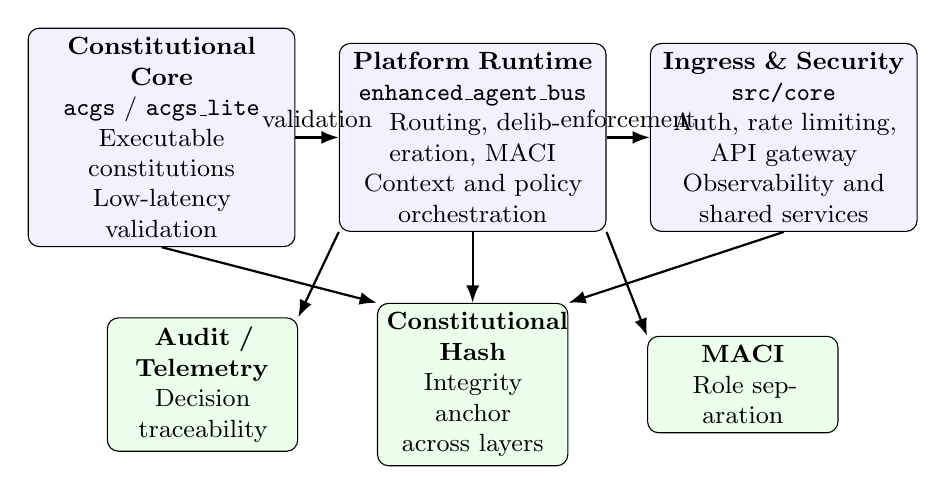
\begin{tikzpicture}[
  font=\small,
  node distance=0.55cm and 0.55cm,
  box/.style={draw, rounded corners, align=center, minimum height=1.15cm, text width=0.26\linewidth, fill=blue!5},
  meta/.style={draw, rounded corners, align=center, minimum height=0.9cm, text width=0.18\linewidth, fill=green!8},
  arr/.style={-{Latex[length=2.2mm]}, thick}
]

\node[box] (core) {\textbf{Constitutional Core}\\\texttt{acgs} / \texttt{acgs\_lite}\\Executable constitutions\\Low-latency validation};
\node[box, right=of core] (runtime) {\textbf{Platform Runtime}\\\texttt{enhanced\_agent\_bus}\\Routing, deliberation, MACI\\Context and policy orchestration};
\node[box, right=of runtime] (ingress) {\textbf{Ingress \& Security}\\\texttt{src/core}\\Auth, rate limiting, API gateway\\Observability and shared services};

\node[meta, below=0.9cm of runtime] (hash) {\textbf{Constitutional Hash}\\Integrity anchor across layers};
\node[meta, left=1.0cm of hash] (audit) {\textbf{Audit / Telemetry}\\Decision traceability};
\node[meta, right=1.0cm of hash] (maci) {\textbf{MACI}\\Role separation};

\draw[arr] (core) -- node[above] {validation} (runtime);
\draw[arr] (runtime) -- node[above] {enforcement} (ingress);
\draw[arr] (core.south) -- (hash.north west);
\draw[arr] (runtime.south) -- (hash.north);
\draw[arr] (ingress.south) -- (hash.north east);
\draw[arr] (runtime.south west) -- (audit.north east);
\draw[arr] (runtime.south east) -- (maci.north west);

\end{tikzpicture}

  }{%
    \fbox{\rule{0pt}{2.1in}\rule{0.92\linewidth}{0pt}}%
  }
  \caption{Architecture overview scaffold. Replace this placeholder with a layered diagram showing the constitutional core (\texttt{acgs}), platform runtime (\texttt{enhanced\_agent\_bus}), and ingress/security surfaces (\texttt{src/core/}), with governance metadata such as constitutional hashes and validation outcomes flowing across layers.}
  \label{fig:architecture-overview}
\end{figure}

\begin{table}[t]
  \centering
  \caption{Claim-tiering scaffold used in this manuscript.}
  \label{tab:claim-tiers}
  \begin{tabular}{p{0.18\linewidth}p{0.24\linewidth}p{0.48\linewidth}}
    \toprule
    Tier & Reporting language & Example use in this paper \\
    \midrule
    Implemented and checked-in & ``implements,'' ``includes,'' ``is represented in the codebase'' & Constitutional hashing across validation, auth, telemetry, and health surfaces \\
    Best-observed benchmark results & ``logged,'' ``best-observed,'' ``under warmed benchmark conditions'' & \texttt{exp254} hot-path throughput and p99 latency \\
    Prototype / research directions & ``prototype,'' ``exploratory,'' ``research direction'' & Mamba-2 long-context modules and broader formal-verification expansion \\
    \bottomrule
  \end{tabular}
\end{table}

\section{Implemented and Checked-In Mechanisms}
This section describes mechanisms that are directly represented in the checked-in repository.

\subsection{Executable Constitutions}
ACGS represents governance policy as structured constitutional artifacts rather than as natural-language prompts alone. Constitutions are loaded from YAML or code-defined builders, compiled into rule structures, and used to evaluate candidate actions. This makes policy evaluation executable, testable, and versionable.

\subsection{Constitutional Hashing and Cryptographic Binding}
A constitutional hash is propagated across multiple validation surfaces as a compact integrity anchor. In the current codebase, the active constitutional hash appears in validation logic, authentication checks, API versioning, OpenTelemetry resource attributes, and health-related surfaces. This design enables downstream components to detect mismatch between the active constitutional artifact and the metadata attached to requests or tokens.

\subsection{Separation of Powers via MACI}
A central governance pattern in ACGS is MACI-style role separation: the actor that proposes or generates an action must not also be the authority that validates it. This design appears throughout the codebase in role definitions, validation pipelines, and governance-oriented processing strategies. Conceptually, the pattern maps onto proposer, validator, and executor responsibilities, reducing the risk of self-approval or self-justification in autonomous workflows.

\subsection{Fail-Closed Policy Enforcement}
The default posture of the system is fail-closed. Validation components are designed so that missing metadata, constitutional hash mismatch, unavailable policy checks, or other governance failures do not silently allow execution. Instead, the system favors deny, block, or escalate behavior depending on the layer and context.

\subsection{Tamper-Evident Audit and Observability}
ACGS includes audit-oriented components and observability hooks intended to make governance decisions inspectable after the fact. The broader platform also propagates constitutional metadata into telemetry and structured events, allowing operators to trace not only what decision was made, but under which constitutional version and enforcement path it was made.

\section{Benchmark Results and Performance Characterization}
This section is limited to benchmarked claims rather than architectural claims.

\subsection{Benchmark Harness}
The repository includes a fixed benchmark harness under \texttt{autoresearch/} for governance-engine optimization. The current checked-in benchmark harness documents \textbf{847 scenarios}, while historical optimization logs in \texttt{autoresearch/results.tsv} include earlier phases using a \textbf{532-scenario} corpus. Accordingly, benchmark numbers should be interpreted in relation to the exact harness revision used.

\subsection{Optimization Trajectory}
The optimization log records \textbf{more than 250 experiments} focused on the Python/Rust hot path. These experiments target matcher behavior, rule precomputation, attribute lookup reduction, warmup strategies, and other low-level performance factors, while preserving correctness constraints such as compliance rate and false-negative rate.

\subsection{Best-Observed Results}
One logged warm-path run (\texttt{exp254}) reports a \textbf{best-observed} configuration with approximately \textbf{1.125M requests per second} and \textbf{p99 latency of 3.92\,$\mu$s}. However, that run is explicitly best-observed rather than a stable promoted baseline: subsequent reruns showed variance, and the corresponding row in the optimization log was not retained as a canonical kept improvement. Repeated kept runs cluster in the \textbf{low-microsecond} range, and optimization notes indicate throughput around \textbf{$\sim$1.1M RPS} under favorable benchmark conditions.

\begin{table}[t]
  \centering
  \caption{Benchmark reporting scaffold. Replace placeholder values with final numbers and hardware metadata for submission.}
  \label{tab:benchmark-summary}
  \begin{tabular}{llll}
    \toprule
    Configuration & Scenario corpus & Throughput (RPS) & p99 latency \\
    \midrule
    Current checked-in harness & 847 scenarios & --- & --- \\
    Historical optimization phase & 532 scenarios & --- & --- \\
    Best-observed warm-path run (\texttt{exp254}) & logged run & $\sim$1.125M & 3.92\,$\mu$s \\
    Repeated kept runs & logged range & $\sim$1.1M & low-\,$\mu$s \\
    \bottomrule
  \end{tabular}
\end{table}

\begin{figure}[t]
  \centering
  \IfFileExists{figures/benchmark_trajectory_placeholder.tex}{%
    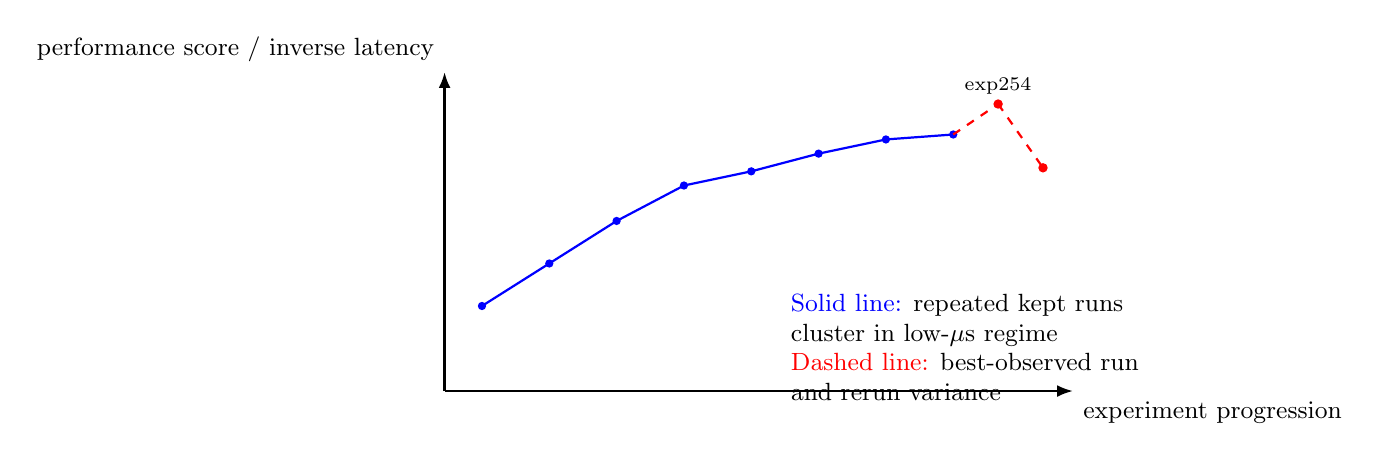
\begin{tikzpicture}[
  font=\small,
  x=0.95cm,
  y=0.9cm,
  axis/.style={thick,-{Latex[length=2mm]}},
  kept/.style={blue, thick},
  outlier/.style={red, thick, dashed},
  note/.style={align=left}
]

% axes
\draw[axis] (0,0) -- (8.4,0) node[below right] {experiment progression};
\draw[axis] (0,0) -- (0,4.5) node[above left] {performance score / inverse latency};

% repeated kept trend
\draw[kept] (0.5,1.2) -- (1.4,1.8) -- (2.3,2.4) -- (3.2,2.9) -- (4.1,3.1) -- (5.0,3.35) -- (5.9,3.55) -- (6.8,3.62);
\foreach \x/\y in {0.5/1.2,1.4/1.8,2.3/2.4,3.2/2.9,4.1/3.1,5.0/3.35,5.9/3.55,6.8/3.62}
  \fill[blue] (\x,\y) circle (1.5pt);

% best-observed point and rerun variance
\draw[outlier] (6.8,3.62) -- (7.4,4.05);
\fill[red] (7.4,4.05) circle (1.7pt);
\draw[outlier] (7.4,4.05) -- (8.0,3.15);
\fill[red] (8.0,3.15) circle (1.7pt);

\node[note, anchor=west] at (4.5,1.0) {\textcolor{blue}{Solid line:} repeated kept runs\\cluster in low-$\mu$s regime};
\node[note, anchor=west] at (4.5,0.2) {\textcolor{red}{Dashed line:} best-observed run\\and rerun variance};
\node[anchor=south] at (7.4,4.05) {\scriptsize exp254};

\end{tikzpicture}

  }{%
    \fbox{\rule{0pt}{1.9in}\rule{0.92\linewidth}{0pt}}%
  }
  \caption{Benchmark characterization scaffold. Suggested replacement: latency distribution or experiment trajectory plot showing the distinction between repeated kept runs and best-observed outliers.}
  \label{fig:benchmark-characterization}
\end{figure}

\subsection{Interpretation}
Table~\ref{tab:benchmark-summary} and Figure~\ref{fig:benchmark-characterization} provide submission-ready scaffolds for reporting benchmark methodology and result dispersion. These results support a narrower and more defensible claim than ``stable sub-4\,$\mu$s production operation.'' Specifically: ACGS demonstrates that deterministic constitutional validation can be implemented with \textbf{microsecond-scale benchmark overhead} on the hot path. At the same time, exact p99 and throughput figures are sensitive to warmup state, interpreter specialization, garbage collection, OS scheduling, and hardware. For this reason, the benchmark should be interpreted as evidence of architectural efficiency, not as a hardware-independent service-level guarantee.

\section{Prototype Modules and Research Directions}
This section separates checked-in prototypes from broader research aspirations.

\subsection{Checked-In Prototype Modules}
The repository contains explicit prototype-oriented work on \textbf{long-context processing} and \textbf{formal verification}:

\begin{itemize}[leftmargin=1.5em]
  \item \textbf{Mamba-2 / Zamba-inspired long-context prototypes} appear in modules such as \texttt{mamba2\_hybrid\_processor.py} and related context-processing code. These modules describe hybrid Mamba-attention architectures and target effective long-context handling~\cite{mamba2,attention}.
  \item \textbf{Z3-based verification components} appear in the verification layer and API surfaces, including a checked-in policy verifier and related metrics and routes. These components indicate an active formal-verification direction already represented in code~\cite{z3}.
\end{itemize}

\subsection{Research-Level Extensions}
Other ideas often associated with the ACGS-2 research lineage should be described more cautiously as \textbf{research directions} unless tied to a concrete checked-in module. These include:

\begin{itemize}[leftmargin=1.5em]
  \item richer temporal reasoning for append-only or history-preserving agents,
  \item broader neuro-symbolic handling of out-of-distribution edge cases,
  \item stronger policy compilation and theorem-proving pipelines beyond the current Z3-oriented work.
\end{itemize}

These directions are consistent with the architecture's goals, but they should not be presented as equally mature with the checked-in constitutional engine or benchmark hot path.

\section{Limitations}
ACGS has several important limitations.

First, the broader platform runtime remains comparatively large and multifunctional. In particular, \texttt{enhanced\_agent\_bus} aggregates responsibilities spanning routing, governance, deliberation, memory, and integration concerns. This creates architectural drag and motivates future decomposition.

Second, maturity varies substantially across subsystems. The constitutional core and benchmark-facing validation path are materially more mature than the long-context and formal-verification prototypes.

Third, benchmark reproducibility is inherently constrained. Peak microsecond-scale measurements are sensitive to hardware, warmup patterns, interpreter specialization, and runtime noise. The strongest reproducible claim is therefore about \textbf{order of magnitude} and \textbf{architectural feasibility}, not a universal fixed latency number.

Finally, constitutional governance infrastructure addresses only one layer of AI system safety. It reduces classes of runtime governance failures, but it does not eliminate risks arising from model capability, data quality, organizational misuse, or flawed downstream procedures.

\section{Discussion}
The broader implication of ACGS is that AI governance can be treated as infrastructure rather than aspiration. In conventional model-centric approaches, rules are frequently encoded as prompt text, moderation heuristics, or fine-tuning objectives. Those mechanisms may shape model behavior, but they are difficult to audit as hard system boundaries. ACGS instead treats constitutions as executable system artifacts with explicit failure modes, integrity metadata, and enforcement paths.

This systems framing also clarifies where different assurances belong. The model is responsible for generation; the governance layer is responsible for boundary enforcement; the runtime is responsible for role separation and execution control; and the audit layer is responsible for traceability. Such decomposition does not solve alignment in the strongest philosophical sense, but it does improve operational governance in settings where evidence, reproducibility, and fail-closed behavior matter.

\section{Conclusion}
ACGS shows that constitutional AI governance can be implemented as executable systems infrastructure rather than as a purely model-internal behavioral objective. In the checked-in implementation, constitutional policies are represented as structured artifacts, validated through fail-closed paths, anchored by constitutional hashes, and enforced across role boundaries. Benchmark results further suggest that this governance layer can operate with microsecond-scale overhead on optimized hot paths, including best-observed throughput above 1.1M RPS under warmed conditions. Just as importantly, the architecture benefits from a clear separation between mature runtime mechanisms and ongoing prototype or research directions. The central lesson is pragmatic: robust AI governance is more credible when it is executable, inspectable, and system-enforced.

\section*{Acknowledgments}
% Optional: add collaborators, reviewers, or funding sources here.

\section*{Artifact and Reproducibility Notes}
This manuscript distinguishes among three classes of claims: (i) implemented and checked-in mechanisms, (ii) benchmarked best-observed results, and (iii) prototype or research directions. Repository-grounded anchors for these claims include \texttt{docs/brand-architecture.md}, \texttt{README.md}, \texttt{autoresearch/benchmark.py}, \texttt{autoresearch/results.tsv}, \texttt{packages/enhanced\_agent\_bus/mamba2\_hybrid\_processor.py}, and \texttt{packages/enhanced\_agent\_bus/verification\_layer/z3\_policy\_verifier.py}.

\bibliographystyle{plain}
\nocite{acgsrepo}
\bibliography{acgs_refs}

\end{document}
